% !TEX root = ../ComputationalOTFnT.tex

\todoK{results about embeddings, Will Leeb's work, Naor's work?}
\todoK{Indyk's embeddings for W1}

\chapter{$\Wass_1$ Optimal Transport}
\label{c-w1}

This chapter focuses on optimal transport problems in which the ground cost is equal to a distance.  Historically, this corresponds to the original problem posed by~\citeauthor{Monge1781} in \citeyear{Monge1781}; this setting was also that chosen in early applications of optimal transport in computer vision~\citep{RubTomGui00} under the name of ``earth mover's distances''.

Unlike the case where the ground cost is a \emph{squared} Hilbertian distance  (studied in particular in Chapter~\ref{c-dynamic}), transport problems where the cost is a metric are more difficult to analyze theoretically.
%
In contrast to Remark~\ref{rem-exist-mongemap} that states the uniqueness of a transport map or coupling between two absolutely continuous measures when using a squared metric, the optimal Kantorovich coupling is in general not unique when the cost is the ground distance itself.  Hence, in this regime it is often impossible to recover a uniquely defined Monge map, making this class of problems ill-suited for interpolation of measures.
%
We refer to works by~\citet{trudinger2001monge,caffarelli2002constructing,sudakov1979geometric,evans1999differential} for proofs of existence of optimal $\Wass_1$ transportation plans and detailed analyses of their geometric structure. 

Although more difficult to analyze in theory, optimal transport with a linear ground distance is usually more robust to outliers and noise than a quadratic cost. Furthermore, a cost that is a metric results in an elegant dual reformulation involving local flow, divergence constraints, or Lipschitzness of the dual potential, suggesting cheaper numerical algorithms that align with \emph{minimum-cost flow} methods over networks in graph theory.
%
This setting is also  popular because the associated OT distances define a norm that can compare arbitrary distributions, even if they are not positive; this property is shared by a larger class of so-called \emph{dual norms} (see \S\ref{sec-dual-norms} and Remark~\ref{rem-unb-dualnorms} for more details).

%%%%%%%%%%%%%%%%%%
\section{$\Wass_1$ on Metric Spaces}
\label{sec-w1-metric}

Here we assume that $d$ is a distance on $\Xx=\Yy$, and we solve the OT problem with the ground cost $c(x,y)=d(x,y)$. The following proposition highlights key properties of the $c$-transform~\eqref{eq-c-transform} in this setup. In the following, we denote the Lipschitz constant of a function $f \in \Cc(\Xx)$ as
\eq{
	\Lip(f) \eqdef \sup \enscond{ \frac{|\f(x)-\f(y)|}{d(x,y)} }{ (x,y) \in \X^2, x \neq y }.
}
We define Lipschitz functions to be those functions $f$ satisfying $\Lip(f) < +\infty$; they form a convex subset of $\Cc(\X)$.

\begin{prop}Suppose $\X=\Y$ and $c(x,y)=d(x,y)$. 
Then, there exists $g$ such that $\f = g^c$ if and only $\Lip(f) \leq 1$. 
Furthermore, if $\Lip(f)\leq1$, then $f^c=-f$.
\end{prop}

\begin{proof}
First, suppose $f=g^c$.  Then, for $x,y\in \X$,
\begin{align*}
|f(x)-f(y)|&=\left|\inf_{z\in\X} d(x,z)-g(z) \;\; - \;\;\inf_{z\in \X} d(y,z)-g(z) \right|\\
&\leq \sup_{z\in\X} |d(x,z)-d(y,z)|\leq d(x,y).
\end{align*}
The first equality follows from the definition of $g^c$, the next inequality from the identity $|\inf f-\inf g|\leq\sup|f-g|$, and the last from the triangle inequality. This shows that $\Lip(f)\leq1$.

Now, suppose $\Lip(f)\leq1$, and define $g\eqdef -f$. By the Lipschitz property, for all $x,y\in\X$,
$f(y)-d(x,y)\leq f(x)\leq f(y)+d(x,y)$.
Applying these inequalities,
\begin{align*}
g^c(y)&=\inf_{x\in\X}\left[ d(x,y) + f(x) \right]
\geq\inf_{x\in \X} \left[  d(x,y)+f(y)-d(x,y)\right]=f(y),\\
g^c(y)&=\inf_{x\in\X}\left[ d(x,y) + f(x) \right]
\leq \inf_{x\in\X}\left[ d(x,y) + f(y)+d(x,y) \right]=f(y).
\end{align*}
Hence, $f=g^c$ with $g=-f$.  Using the same inequalities shows
\begin{align*}
f^c(y)&=\inf_{x\in\X}\left[ d(x,y) - f(x) \right]
\geq\inf_{x\in \X} \left[  d(x,y)-f(y)-d(x,y)\right]=-f(y),\\
f^c(y)&=\inf_{x\in\X}\left[ d(x,y) - f(x) \right]
\leq \inf_{x\in\X}\left[ d(x,y) - f(y)+d(x,y) \right]=-f(y).
\end{align*}
This shows $f^c=-f$.
\end{proof}

Starting from the single potential formulation~\eqref{eq-semi-dual-cont}, one can iterate the construction and replace the couple $(\g,\g^c)$ by $(\g^c,(\g^c)^c)$. The last proposition shows that one can thus use $(\g^c,-\g^c)$, which in turn is equivalent to any pair $(f,-f)$ such that $\Lip(f) \leq 1$. This leads to the following alternative expression for the $\Wass_1$ distance:
%Plugging the relationship $f^c=-f$ into~\eqref{eq-semi-dual-cont} shows
\eql{\label{eq-w1-metric}
	\Wass_1(\al,\be) = 
	\umax{f} \enscond{ \int_{\Xx} f(x) (\d\al(x)-\d\be(x)) }{ \Lip(f) \leq 1 }.
}
This expression shows that $\Wass_1$ is actually a norm, \ie $\Wass_1(\al,\be) = \norm{\al-\be}_{\Wass_1}$, and that it is still valid for any measures (not necessary positive) as long as $\int_{\Xx} \al=\int_{\Xx} \be$.  This norm is often called the \citeauthor{kantorovich1958space} norm~\citeyearpar{kantorovich1958space}.

For discrete measures of the form~\eqref{eq-discr-meas}, writing $\al-\be = \sum_{k} \VectMode{m}_k \de_{z_k}$ with $z_k \in \Xx$ and $\sum_k \VectMode{m}_k=0$, the optimization~\eqref{eq-w1-metric} can be rewritten as
\eql{\label{eq-w1-discr}	
	\Wass_1(\al,\be) = 
	\umax{ (\fD_k)_k } \enscond{ \sum_k \fD_k \VectMode{m}_k }{ \foralls (k,\ell), 
		\abs{\fD_k-\fD_\ell} \leq d(z_k,z_\ell), }
}
which is a finite-dimensional convex program with quadratic-cone constraints.  It can be solved using interior point methods or, as we detail next for a similar problem, using proximal methods. 

When using $d(x,y)=|x-y|$ with $\X=\RR$, we can reduce the number of constraints by ordering the $z_k$'s via $z_1 \leq z_2 \leq \ldots$.  In this case, we only have to solve
\eq{	
	\Wass_1(\al,\be) = 
	\umax{ (\fD_k)_k } \enscond{ \sum_k \fD_k \VectMode{m}_k }{ \foralls k, \abs{\fD_{k+1}-\fD_k} \leq z_{k+1}-z_k }, 
}
which is a linear program. 
%
Note that furthermore, in this 1-D case, a closed form expression for $\Wass_1$ using cumulative functions is given in~\eqref{eq-w1-1d}.

\begin{rem}[$\Wass_p$ with $0<p \leq 1$]
	If $0<p \leq 1$, then $\tilde d(x,y) \eqdef d(x,y)^p$ satisfies the triangular inequality, and hence $\tilde d$ is itself a distance. One can thus apply the results and algorithms detailed above for $\Wass_1$ to compute $\Wass_p$ by simply using $\tilde d$ in place of $d$. This is equivalent to stating that $\Wass_p$ is the dual of $p$-H\"older functions $\ensconds{f}{\Lip_p(f) \leq 1}$, where
	\eq{
		\Lip_p(f) \eqdef \sup \enscond{ \frac{|\f(x)-\f(y)|}{d(x,y)^p} }{ (x,y) \in \X^2, x \neq y }.
	}
\end{rem}

%%%%%%%%%%%%%%%%%%
\section{$\Wass_1$ on Euclidean Spaces}
\label{sec-w1-eucl}


In the special case of Euclidean spaces $\X=\Y=\RR^\dim$, using $\c(x,y) = \norm{x-y}$, the global Lipschitz constraint appearing in~\eqref{eq-w1-metric} can be made local as a uniform bound on the gradient of $f$, 
\eql{\label{eq-w1-cont}
	\Wass_1(\al,\be) = 
	\umax{f} \enscond{ \int_{\RR^\dim} \f(x) (\d\al(x)-\d\be(x)) }{ \norm{\nabla \f}_\infty \leq 1 }.
}
Here the constraint $\norm{\nabla \f}_\infty \leq 1$ signifies that the norm of the gradient of $\f$ at any point $x$ is upper bounded by $1$, $\norm{\nabla \f(x)}_2 \leq 1$ for any $x$.

Considering the dual problem to~\eqref{eq-w1-cont}, one obtains an optimization problem under fixed divergence constraint
\eql{\label{eq-w1-cont-div}
	\Wass_1(\al,\be) = 
	\umin{\flow} \enscond{ \int_{\RR^\dim} \norm{\flow(x)}_2 \d x }{  \diverg(\flow)=\al-\be }, 
}
which is often called the Beckmann formulation~\citep{Beckmann52}.
%
Here the vectorial function $\flow(x) \in \RR^2$ can be interpreted as a flow field, describing locally the movement of mass. Outside the support of the two input measures, $\diverg(\flow)=0$, which is the conservation of mass constraint. 
%
Once properly discretized using finite elements, Problems~\eqref{eq-w1-cont} and~\eqref{eq-w1-cont-div} become nonsmooth convex optimization problems. 
%
It is possible to use an off-the-shelf interior points quadratic-cone optimization solver, but as advocated in~\S\ref{sec-prox-solvers}, large-scale problems require the use of simpler but more adapted first order methods. One can thus use, for instance, Douglas--Rachford (DR) iterations~\eqref{eq-dr-iters} or the related alternating direction method of multipliers method. Note that on a uniform grid, projecting on the divergence constraint is conveniently handled using the fast Fourier transform. We refer to~\citet{SolomonEMDSurfaces2014} for a detailed account for these approaches and application to OT on triangulated meshes.
%
See also~\citet{LiRyuOsherYinGangbo2017_parallel,Ryu2017a,Ryu2017b} for similar approaches using primal-dual splitting schemes.
%
Approximation schemes that relax the Lipschitz constraint on the dual potentials $\f$ have also been proposed, using, for instance, a constraint on wavelet coefficients leading to an explicit formula~\citep{shirdhonkar2008approximate}, or by considering only functions $\f$ parameterized as multilayer neural networks with ``rectified linear'' $\max(0,\cdot)$ activation function and clipped weights~\citep{WassersteinGAN}.

%%%%%%%%%%%%%%%%%%
% \section{$\Wass_1$ on Smooth Manifolds}
% \label{sec-w1-manifolds}


%%%%%%%%%%%%%%%%%%
\section{$\Wass_1$ on a Graph}

The previous formulations~\eqref{eq-w1-cont} and~\eqref{eq-w1-cont-div} of $\Wass_1$ can be generalized to the setting where $\X$ is a geodesic space, \ie $\c(x,y)=\dist(x,y)$ where $\dist$ is a geodesic distance. We refer to~\citet{FeldmanMacCann02} for a theoretical analysis in the case where $\X$ is a Riemannian manifold.
%
When $\X=\range{1,n}$ is a discrete set, equipped with undirected edges $(i,j) \in \Edges \subset \X^2$ labeled with a weight (length) $\weight_{i,j}$, we recover the important case where $\X$ is a graph equipped with the geodesic distance (or shortest path metric):
\eq{
	\distD_{i,j} \eqdef \umin{K \geq 0, (i_k)_k : i \rightarrow j }
	 \enscond{ \sum_{k=1}^{K-1} \weight_{i_k,i_{k+1}} }{ \foralls k \in \range{1,K-1}, (i_k,i_{k+1}) \in \Ee  },
}
where $i \rightarrow j$ indicates that $i_1=i$ and $i_K=j$, namely that the path starts at $i$ and ends at $j$.

We consider two vectors $(\a,\b) \in (\RR^n)^2$ defining (signed) discrete measures on the graph $\X$ such that $\sum_i \a_i = \sum_i \b_i$ (these weights do not need to be positive). 
%
The goal is now to compute $\WassD_1(\a,\b)$, as introduced in~\eqref{eq-wass-p-disc} for $p=1$, when the ground metric is the graph geodesic distance. This computation should be carried out without going as far as having to compute a ``full'' coupling $\P$ of size $n \times n$, to rely instead on local operators thanks to the underlying connectivity of the graph. These operators are discrete formulations for the  gradient and divergence differential operators.

A discrete dual Kantorovich potential $\fD \in \RR^n$ is a vector indexed by all vertices of the graph. The gradient operator $\nabla : \RR^n \rightarrow \RR^{\Edges}$ is defined as
\eq{
	\foralls (i,j) \in \Edges, \quad (\nabla \fD)_{i,j} \eqdef \fD_i-\fD_j.
}
A flow $\flowD = (\flowD_{i,j})_{i,j}$ is defined on edges, and the divergence operator $\diverg : \RR^{\Edges} \rightarrow \RR^n$, which is the adjoint of the gradient $\nabla$, maps flows to vectors defined on vertices and is defined as
\eq{
	\foralls i \in \range{1,n}, \quad \diverg(\flowD)_i \eqdef \sum_{j: (i,j) \in \Edges} (\flowD_{i,j} - \flowD_{j,i}) \in \RR^n.
}


Problem~\eqref{eq-w1-cont} becomes, in the graph setting, 
\eql{\label{eq-w1-graph-potential}
	\WassD_1(\a,\b) = 
	\umax{\fD \in \RR^n} \enscond{ \sum_{i=1}^n \fD_i (\a_i-\b_i)   }{  \forall (i,j) \in \Edges, \, |(\nabla \fD)_{i,j}| \leq \weight_{i,j}  }.
}
The associated dual problem, which is analogous to Formula~\eqref{eq-w1-cont-div}, is then
\eql{\label{eq-w1-graph-div}
	\WassD_1(\a,\b) = 
	\umin{\flowD \in \RR_+^\Edges} \enscond{ \sum_{(i,j) \in \Ee} \weight_{i,j} \flowD_{i,j}  }{  \diverg(\flowD)=\a-\b }.
}
This is a linear program and more precisely an instance of min-cost flow problems. Highly efficient dedicated simplex solvers have been devised to solve it; see, for instance,~\citep{TreeEMD2007}. % \todoK{detail this}
% 
Figure~\ref{fig-planar-graph} shows an example of primal and dual solutions. 
%
Formulation~\eqref{eq-w1-graph-div} is the so-called Beckmann formulation~\citep{Beckmann52} and has been used and extended to define and study traffic congestion models; see, for instance,~\citep{CarlierSantambrogioOTCongestion2008}.

 


\begin{figure}[h!]
\centering
\begin{tabular}{@{}c@{\hspace{10mm}}c@{}}
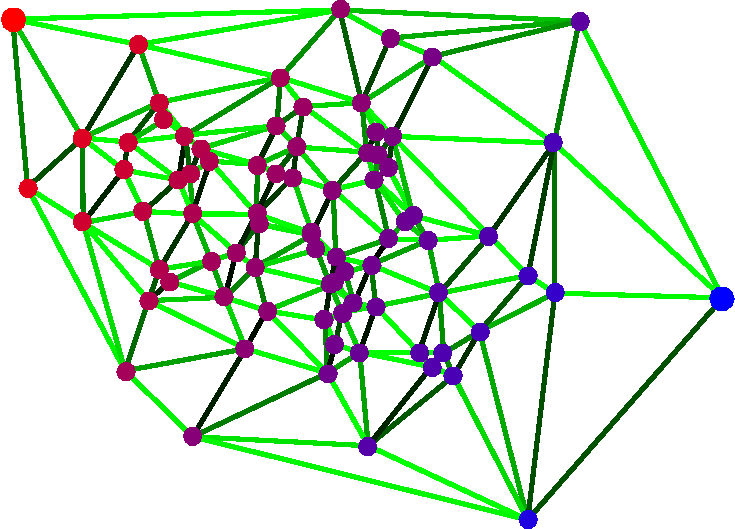
\includegraphics[width=.45\linewidth]{w1-graph/potential}&
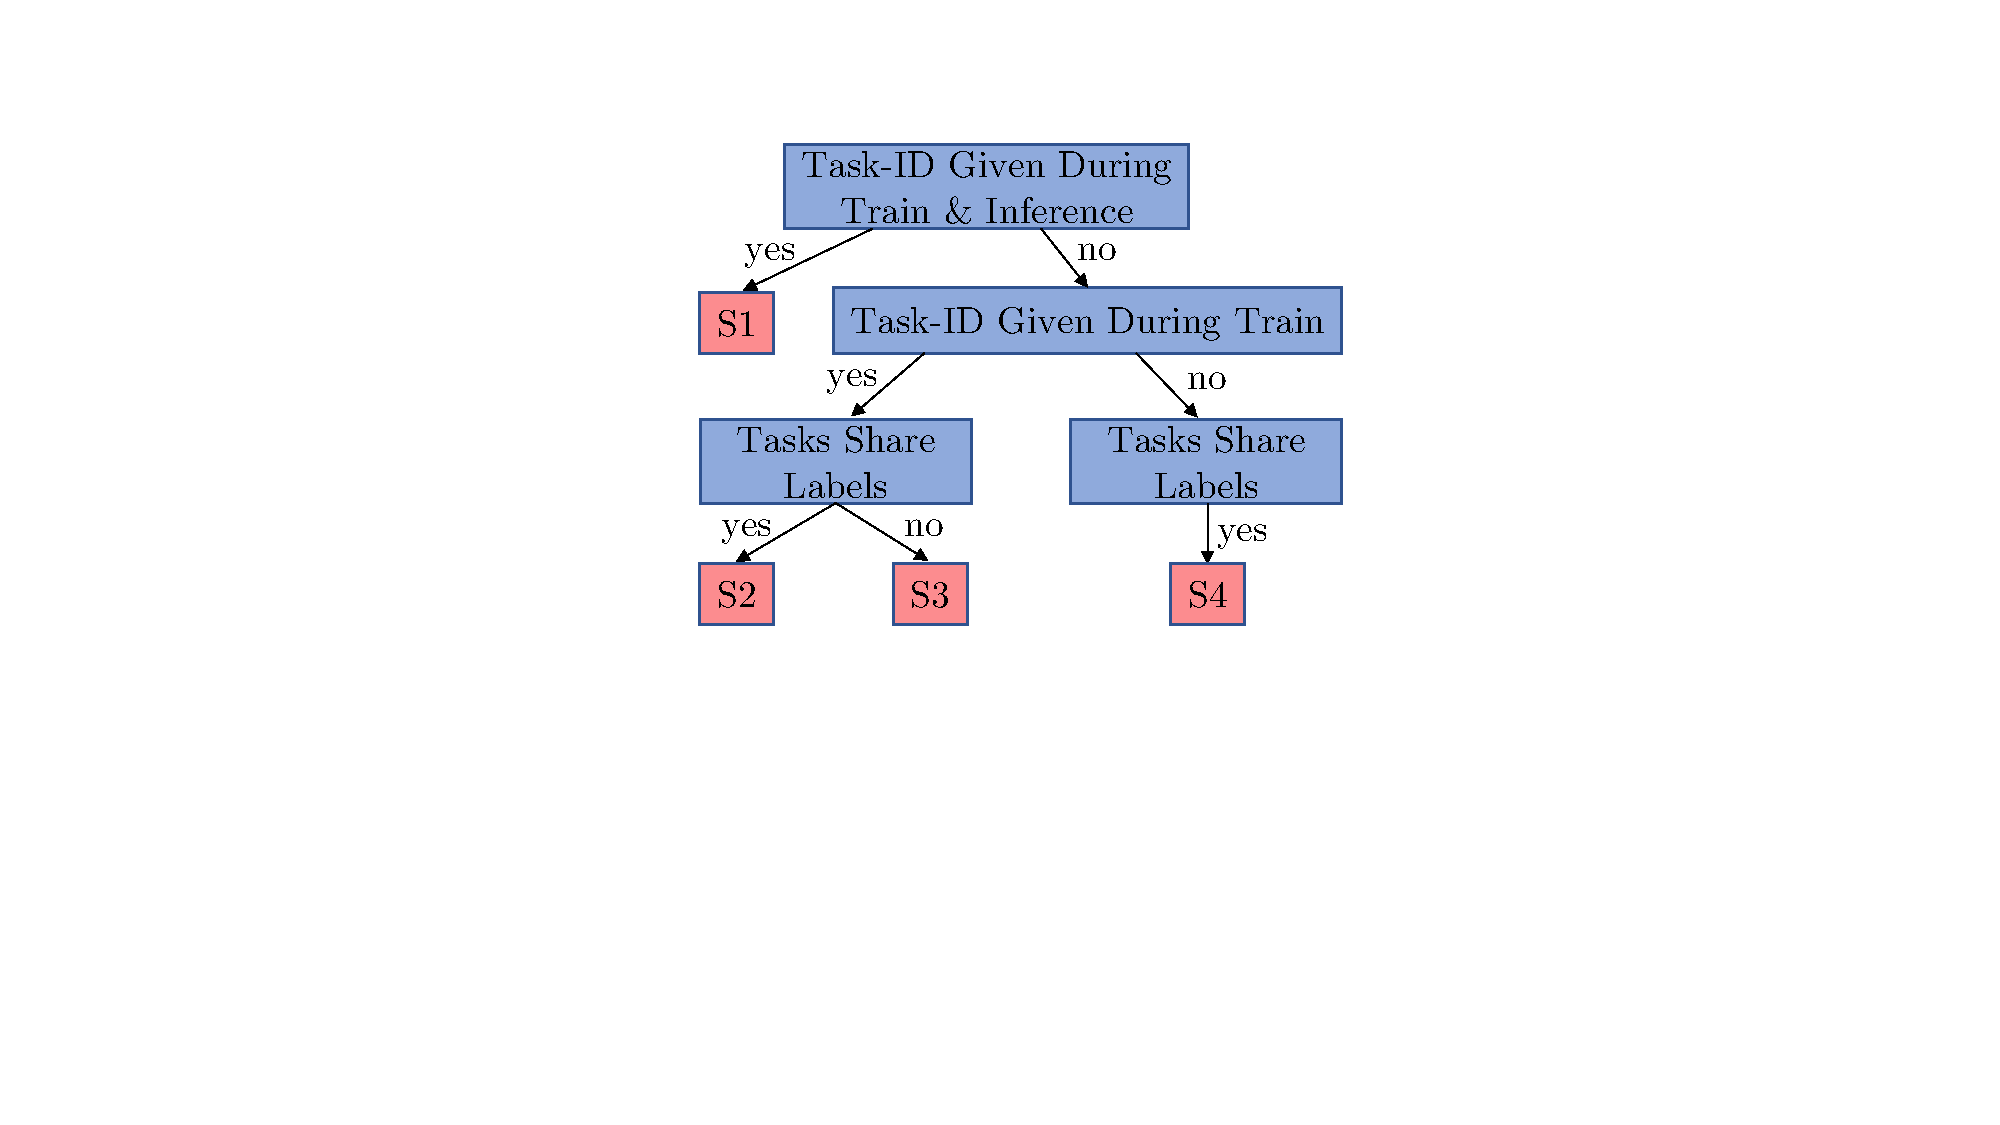
\includegraphics[width=.45\linewidth]{w1-graph/flow}\\
$\fD$ & $({\color{red}\a},{\color{blue}\b})$ and $\flowD$ 
\end{tabular}
\caption{\label{fig-planar-graph}
Example of computation of $\WassD_1(\a,\b)$ on a planar graph with uniform weights $\weight_{i,j}=1$.
%
Left: potential $\fD$ solution of~\eqref{eq-w1-graph-potential} (increasing value from red to blue). The green color of the edges is proportional to $|(\nabla \fD)_{i,j}|$. 
%
Right: flow $\flowD$ solution of~\eqref{eq-w1-graph-div}, 
where bold black edges display nonzero $\flowD_{i,j}$, which saturate to $\weight_{i,j}=1$.
%
These saturating flow edge on the right match the light green edge on the left where $|(\nabla \fD)_{i,j}|=1$.
}
\end{figure}





